\clearpage
\section{光谱、色散、球谐函数与体素}
\subsection*{从一束光到屏幕颜色}

一面白墙在暖灯下微微发黄。灯发出了什么光，墙又把其中多少光反射到了眼前？把光按波长展开，就得到它的光谱\term{spectrum}。横轴上的波长常用纳米（nm）表示，纵轴告诉我们在各波长附近有多少光。光源可以在许多波长上都有输出，也可以把大部分能量集中在很窄的一段。同样明亮的两盏灯，光谱的形状也可能很不一样。

先只比较两个同样宽的窄波段。假设蓝光附近和红光附近各有 4 份光落在一块颜料上。颜料在蓝光附近反射四分之一，在红光附近反射四分之三。于是反射出去的蓝光有 1 份，红光有 3 份。这个算法可以对每一小段波长分别做一次。用 $\lambda$ 表示波长，$S_{\rm in}$ 表示落在表面的光谱，$\rho$ 表示该波长的反射比例。对普通的漫反射颜料，把各波长相同的几何因素暂时略去，有
\[
  S_{\rm out}(\lambda)=S_{\rm in}(\lambda)\,\rho(\lambda).
\]
\begin{center}
\small
\begin{tabular}{@{}lrrr@{}}
\toprule
比较的窄波段 & 落在颜料上的光 & 反射比例 & 反射出去的光 \\
\midrule
450 nm 附近（蓝）& 4 份 & $1/4$ & 1 份\\
650 nm 附近（红）& 4 份 & $3/4$ & 3 份\\
\bottomrule
\end{tabular}
\end{center}

显示器需要的是红、绿、蓝三个数。可以先用三条颜色匹配曲线对光谱分别做加权求和，得到标准颜色空间 CIE XYZ 中的三个数，再换算成显示用的 RGB。例如 $Y$ 对应人眼在明亮环境下的亮度响应，$\bar y(\lambda)$ 是不同波长的权重，$k$ 取决于使用的单位。下面的积分就是把每一小段波长的贡献相加。
\[
  Y=k\int_{\text{可见光}} S_{\rm out}(\lambda)\,\bar y(\lambda)\,{\rm d}\lambda .
\]
三次求和会丢失细节。两块色样在一盏灯下可以看成同色，换一盏光谱不同的灯，各波长参加求和的比重变了，色样就可能显出差别。

再回到编辑器里的那面墙。底色贴图已经把颜色存成 RGB，GI 着色器把读到的 sRGB 转为线性值，便可将底色与灯光逐分量相乘。假设灯光是 $(1,0.5,0.25)$，墙面刷上 $(0.8,0.4,0.2)$ 的漆，乘完得到 $(0.8,0.2,0.05)$，之后还要考虑入射角和距离。把墙重新刷白，三个分量就能保留更多灯光原有的颜色。若想预测两块同色的漆换灯之后能否分辨出来，仅有这三个数已经不够，还需要颜料和灯光的光谱。

\noindent{\small\color{quiet} 对照阅读\enspace
\href{https://pbr-book.org/4ed/Radiometry,_Spectra,_and_Color/Representing_Spectral_Distributions}{PBRT 第四版 §4.5，图 4.16 柠檬皮的反射曲线}；
\href{https://pbr-book.org/4ed/Radiometry,_Spectra,_and_Color/Color}{§4.6，图 4.18 颜色匹配曲线}。
项目入口是 \href{run:../../Redflag/src/Redflag/Renderer/GI/Shaders/GI.comp}{GI.comp} 的 \texttt{linearTexel} 和 \texttt{direct}。}

\clearpage
\subsection*{棱镜中的色散}

把一束窄的白光射入玻璃棱镜，另一侧能看到颜色逐渐展开。白光本来就包含许多波长。普通玻璃对不同波长有略微不同的折射率 $n(\lambda)$，光从空气斜着进入玻璃时，各波长在界面处转过的角度便有细小差别。这种光学性质称为色散\term{dispersion}。

\begin{center}
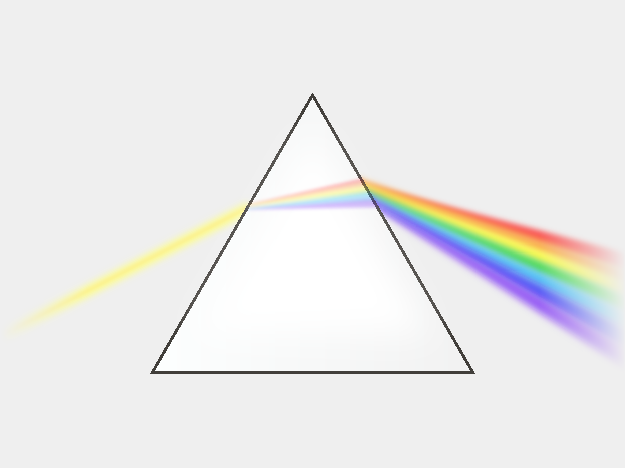
\includegraphics[width=.48\linewidth]{figures/prism-rainbow.pdf}\\[-1pt]
{\small 从入射光束沿玻璃向右看，出射一侧可以分辨不同波长的方向。}\\
{\footnotesize\color{quiet}\href{https://commons.wikimedia.org/wiki/File:Prism-rainbow.svg}{Suidroot，\emph{Prism-rainbow}，2008}，
\href{https://creativecommons.org/licenses/by-sa/4.0/}{CC BY-SA 4.0}。原图转为 PDF。}
\end{center}

角度要从界面的法线量起。法线就是穿过入射点、垂直于玻璃表面的直线。设入射角为 $\theta_i$，进入玻璃后的角为 $\theta_t$，斯涅尔定律写作
\[
  n_{\text{空气}}\sin\theta_i=n_{\text{玻璃}}(\lambda)\sin\theta_t(\lambda).
\]
取空气折射率为 1，让入射角等于 $30^\circ$，左边就是 $1/2$。为了看清差别，把红光和蓝光的折射率分别取为 $1.50$ 和 $1.60$，这组教学数值放大了色散。红光在玻璃里的角度满足 $\sin\theta_t=1/3$，约为 $19.5^\circ$。蓝光得到 $5/16$，约为 $18.2^\circ$，在这里更靠近法线。棱镜的第二个面与第一个面不平行，出射后两束光沿不同方向前进，在远处的屏上就能分开。

设想用渲染器把这束光一直追到白屏上。红光射到屏幕的哪个点，要用红光的折射率穿过两道玻璃表面才能知道，蓝光则要用它自己的折射率再算一遍。等各波长到达各自的像素，才合成为屏幕颜色。前面照亮墙面的 RGB 漫反射在同一条光路上计算三个分量。当前引擎还没有沿不同波长分别追踪玻璃折射的步骤。

\noindent{\small\color{quiet} 同一玻璃场景的两次渲染见
\href{https://pbr-book.org/4ed/Reflection_Models/Specular_Reflection_and_Transmission}{PBRT 第四版 §9.3.1，图 9.9}。比较玻璃投下的亮斑，可以看到固定折射率和随波长变化的折射率给出的差别。}

\clearpage
\subsection*{窗边的石膏球}

把一个灰色石膏球搬到窗边。朝向天空的一面较亮，朝向地面的一面较暗。给球着色时，光是知道球心在窗边还不够，还要知道每一小块球面朝向哪里。第~\ref{lesson-ddgi}~章的探针在窗旁取样时，以世界坐标的六个正负轴为中心，分别向对应半球发射光线，留下六组 RGB 平均值和命中距离统计。

给石膏球的顶端着色，程序只取 $+y$ 那一组。走到斜面，法线 $n$ 恰好在 $+x$ 与 $+y$ 之间，每组按 $\max(0,n\cdot a)^2$ 参与，其中 $a$ 是这一组的轴向。这两组各占 $(1/\sqrt2)^2=1/2$。石膏球放在几个探针之间时，还要结合距离和遮挡混合附近八个探针。整个计算直接读取各方向的值。

也可以把天空的明暗看成一幅铺在单位球面上的图。用 $\omega$ 表示从球心指向球面的单位方向，以 $+y$ 为上，假设一个颜色分量的亮度是 $L(\omega)=2+\omega_y$。这个图样可以分两笔画成。先把整个球涂成亮度 2，再叠加一层从下往上逐渐变亮的图样。在下方，第二笔让原来的亮度减去 1。

\begin{center}
\begin{tikzpicture}[x=.77cm,y=.67cm,font=\small]
  \draw[quiet!35] (0,0) circle[x radius=1.38,y radius=1.38];
  \foreach \a/\b in {0/1.26,1.26/0,0/-1.26} \draw[->,thick,wine] (0,0)--(\a,\b);
  \fill[ink] (0,0) circle (2pt);
  \node[anchor=east] at (-1.55,0) {探针};
  \draw[quiet] (-1.42,0)--(-.16,0);
  \node[anchor=west] at (.44,1.17) {向上\quad $2+1=3$};
  \node[anchor=west] at (1.62,0) {水平\quad $2+0=2$};
  \node[anchor=west] at (.44,-1.17) {向下\quad $2-1=1$};
\end{tikzpicture}\\
{\small 本册绘制。在同一个探针位置，向三个方向读取例子里的亮度。}
\end{center}

球谐函数\term{spherical harmonics, SH}给出了一套可以这样叠加的球面函数。最低一层处处相同，下一层描述三个方向上的渐变，再下一层还能表示更细的起伏。用 $Y_{\ell m}$ 记第 $\ell$ 层中的一个函数，$c_{\ell m}$ 记它在当前光照里占多少。选取正交归一的实球谐基时，前三层的近似为
\[
 c_{\ell m}=\int_{S^2}L(\omega)Y_{\ell m}(\omega)\,{\rm d}\omega ,
 \qquad
 L(\omega)\approx\sum_{\ell=0}^{2}\ \sum_{m=-\ell}^{\ell} c_{\ell m}Y_{\ell m}(\omega).
\]
左边沿整个球面求和，计算光照与每一种分布的吻合程度。右边在所问方向上把它们加回来。三层各有 $1,3,5$ 个函数，每个颜色分量需要 9 个系数。前面例子里的 $2$ 和 $1$ 是常数和方向余弦的倍率，换成归一化的球谐基时倍率会相应换算。漫反射表面汇集来自一大片方向的光，把细小的亮暗变化抹平，因而适合这种低阶近似。若要保留镜面里一颗很小的太阳，九个数就太少了。换成一颗金属球，粗糙度还会改变倒影的清晰程度。配套的\href{run:Redflag-Rendering-Math.pdf}{《渲染公式与实现》}用 OpenGL 的环境贴图来画这种表面。

\noindent{\small\color{quiet} \href{https://graphics.stanford.edu/papers/envmap/}{Ramamoorthi 与 Hanrahan，漫反射环境光的球谐近似（2001）}；
\href{https://sites.cs.ucsb.edu/~lingqi/teaching/resources/GAMES202_Lecture_06.pdf}{闫令琪，GAMES202 第六讲球谐基图示}。
\href{run:../../Redflag/src/Redflag/Renderer/GI/Shaders/GI.comp}{项目实现}见 \texttt{updateProbe} 和 \texttt{gatherProbes}。}

\clearpage
\subsection*{墙面与体素}

一束光穿过房间，最后碰到墙。前面的间接光算法要找准确的撞击点，于是用包围盒树（BVH）先跳过整组碰不到的三角形，再对剩下的三角形求交。换个问题，若只关心“房间的哪一小块空间被墙占着”，可以预先把空间切成等大的小立方体，在与墙面相交的格子里留下标记。这样的三维格子叫作体素\term{voxel}，把三角形模型写入这些格子的过程就叫体素化。

设格网原点为 $(0,0,0)$，每格边长 $h=0.5$ 米。要找墙上一点 $p=(1.2,0.3,0.8)$ 米落在哪一格，先用各坐标除以边长，再分别向下取整。这样得到从 0 开始数的格号。
\[
 (i_x,i_y,i_z)=\lfloor p/h\rfloor
   =\lfloor(2.4,0.6,1.6)\rfloor=(2,0,1).
\]
\begin{center}
\begin{tikzpicture}[x=.78cm,y=.78cm,font=\small]
  \fill[wine!17] (2,1) rectangle (3,2);
  \draw[step=1,gray!65] (0,0) grid (4,3);
  \draw[->,thick] (0,0)--(4.38,0) node[right] {$x$};
  \draw[->,thick] (0,0)--(0,3.36) node[above] {$z$};
  \foreach \x in {0,1,2,3} \node[below] at (\x+.5,0) {\x};
  \foreach \z in {0,1,2} \node[left] at (0,\z+.5) {\z};
  \fill[wine] (2.4,1.6) circle (3pt);
  \draw[wine] (2.4,1.6)--(4.8,2.05)--(5.2,2.05);
  \node[anchor=west] at (5.2,2.05) {墙上的点 $p$};
  \node[anchor=west,text=quiet] at (5.2,1.2) {淡红色表示它落入的格子};
\end{tikzpicture}\\
{\small 本册绘制。从上方看第 $i_y=0$ 层。坐标轴下方和左边标出格号，每格宽半米。}
\end{center}

若按 $x$ 最快、其次 $y$、最后 $z$ 的顺序存储，设每行有 4 个格子，每层有 3 行，格号 $(2,0,1)$ 的数组下标就是 $2+4(0+3\times1)=14$。格子越小，斜墙的轮廓越贴近原来的三角形。若把三个方向都细分一倍，并给每个格子分配存储，格数就增为 $2^3=8$ 倍。稀疏结构只为需要记录的区域分配空间，可以减轻这项开销。

现在在窗前添一小团烟。若每格记录烟的密度，就可以沿光路一格一格地读。假设前三格一样厚，光在各格穿出后分别剩下进入时的全部、一半和一半。那么 4 份光穿过第一格仍有 4 份，穿过第二格剩 2 份，穿过第三格就只剩 1 份。这里每一格都代表房间里的固定位置，转动相机后烟仍在原处。第~\ref{lesson-cluster}~章给点光源分簇时也能看到格子，但那些格子随相机移动，存的是哪些灯可能照到画面的这一块。当前引擎靠三角形求墙面交点，例子里的密度格网则是画烟时可以另选的一种表示。

\noindent{\small\color{quiet} \href{https://michael-schwarz.com/research/publ/2010/vox/}{Schwarz 与 Seidel，三角网格的体素化（2010）}；
\href{https://pbr-book.org/4ed/Volume_Scattering/Media}{PBRT 第四版 §11.4，格网介质}；
\href{run:../../Redflag/src/Redflag/Renderer/GI/GIScene.cpp}{项目包围盒树}；
\href{run:../../Redflag/src/Redflag/Renderer/ScreenSpace/Shaders/Cluster.glsl}{屏幕分簇的下标与深度}。}
